
% !TeX spellcheck = en_US
\documentclass{article}
\usepackage[english]{babel}
\usepackage[utf8]{inputenc}
\usepackage{fancyhdr}
\usepackage{xcolor}
\usepackage{lmodern}
\usepackage{listings}
\usepackage{amsmath}
\usepackage{amssymb}
\usepackage{graphicx}
\usepackage{physics}
\lstset{language=[90]Fortran,
	basicstyle=\ttfamily,
	keywordstyle=\color{blue},
	commentstyle=\color{green},
	morecomment=[l]{!\ }% Comment only with space after !
}

\usepackage{color}
\definecolor{deepblue}{rgb}{0,0,0.5}
\definecolor{deepred}{rgb}{0.6,0,0}
\definecolor{deepgreen}{rgb}{0,0.5,0}

% Default fixed font does not support bold face
\DeclareFixedFont{\ttb}{T1}{txtt}{bx}{n}{10} % for bold
\DeclareFixedFont{\ttm}{T1}{txtt}{m}{n}{10}  % for normal

% Python style for highlighting
\lstset{
	language=Python,
	basicstyle=\ttm,
	otherkeywords={self},             % Add keywords here
	keywordstyle=\ttb\color{deepblue},
	emph={__init__},          % Custom highlighting
	emphstyle=\ttb\color{deepred},    % Custom highlighting style
	stringstyle=\color{deepgreen},
	frame=tb,                         % Any extra options here
	showstringspaces=false            % 
}





\pagestyle{fancy}
\fancyhf{}
\lhead{Vincenzo Maria Schimmenti - 1204565}
\rhead{\today}
\rfoot{Page \thepage}
\lfoot{Exercise 9}
\title{%
	Information Theory and Computation \\
	Exercise  9}
\author{Vincenzo Maria Schimmenti - 1204565}
\begin{document}
\maketitle
 
\section*{Theory}
In this exercise we are gonna diagonalize the Quantum Ising model with the Hamiltonian:
\begin{equation}
	H=\lambda \sum_{i=1}^N \sigma^z_i + \sum_{i=1}^{N-1} \sigma^x_i \sigma^x_{i+1}
\end{equation}
As a basis for the one particle Hilbert space we chose the one diagonalizing $\sigma^z$:
\begin{flalign}
	& \sigma^z \ket{0}=\ket{0} \\
	& \sigma^z \ket{1}=-\ket{1}
\end{flalign}
An $N-$particles wave function is defined by a family of $\{n_i\} n_i=0,1$ i.e.
\begin{equation}
	\ket{n_1} \ket{n_2} \dots \ket{n_M}
\end{equation}
We can observe that there is a one to one correspondence between a wavefunction and an integer number form $0$ to $2^N-1$; from the coefficients above we obtain the number by computing:
\begin{equation}
	n_1+n_2 \times 2+n_3 \times 2^2 + \dots + n_N \times 2^{N-1}
\end{equation}
In other words, we treat the sequence $n_N n_{N-1} \dots n_1$ as a binary number. Since we chose the diagonal basis the action of $\sum_{i=1}^N \sigma_i^z$ on a $N$ particles state is trivial; instead $\sigma^x_i \sigma^x_{i+1}$ as as:
\begin{equation}
	\sigma^x_i \sigma^x_{i+1} \ket{n_1} \ket{n_2} \dots \ket{n_M} = \ket{n_1} \ket{n_2} \dots \ket{1-n_i} \ket{1-n_{i+1}} \dots  \ket{n_M}
\end{equation}
i.e. flips the $i$-th and the $i+1$-th spin. Denoting $\ket{m}=\ket{m_1 m_2 \dots m_N}$ and $\ket{n}=\ket{n_1 n_2 \dots n_N}$ with $m$ and $n$ constructed as above said, the matrix element  $\bra{m} \sigma^x_i \sigma^x_{i+1} \ket{n}$ is non zero if and only if the numbers $m$ and $n$, in binary, have the same digits apart from the $i$-th and $i+1$-th, where they must be opposite; one can express this property by the following predicate:
\begin{equation}
	\bra{m} \sigma^x_i \sigma^x_{i+1} \ket{n} \neq 0 \leftrightarrow \text{XOR}(n, 3\times 2^{i-1})==m
\end{equation}
The $\text{XOR}$ operation is done logically, bit-by-bit. The above property can be used to compute the Hamiltonian matrix elements:
\begin{equation}
	H_{m,n} = \bra{m} H \ket{n} = \lambda \delta_{m,n} + \sum_{i=1}^{N-1} \delta_{m,\text{XOR}(n, 3\times 2^{i-1})}
\end{equation}
The number $3 \times 2^{i-1}$ is a \textit{mask} number, useful to compare the bits of each index $m$ and $n$: it is equal to the binary $11_2$ shifted towards the left in order to force the $i$-th nd $i+1$-th bits to be opposite (an the others to be equal). Practically, given some $m$, look for all the $n$'s that have non zero $\delta_{m,\text{XOR}(n, 3\times 2^{i-1})}$, for $i=1 \dots N-1$.
\section*{Code Development}
Essentially we need two function to build the Hamiltonian; the first one is the function computing the magnetization for a given state (i.e. the first part of the Hamiltonian); basically, for a state indexed by the number $n$, the magnetization is given by the number of zeros minus the number of ones in the binary representation:
\begin{lstlisting}[language=Fortran]
function magnetization_integer(x, N)result(mgn)
	integer*4, intent(in) :: x,N
	integer*4 :: ii, mgn
	mgn = 0
	do ii=0,N-1
		if(BTEST(x, ii))then
			mgn = mgn - 1
		else
			mgn = mgn + 1
		end if
	end do
end function
\end{lstlisting}
The second function we need is the one that actually computes the Hamiltonian matrix elements:
\begin{small}
\begin{lstlisting}[language=Fortran]
function isingHamiltonian(N,lmbd)result(H)
	integer*4, intent(in) :: N
	real*8, intent(in) :: lmbd
	complex*16, dimension(:,:), allocatable :: H
	integer*4 :: sz,mm,nn,mask,kk
	sz = 2**N
	allocate(H(sz,sz))
	H = 0
	do mm=0,sz-1
		H(mm+1,mm+1)=lmbd*magnetization_integer(mm, N)
		mask = 3
		do kk=1,N-1
			nn = xor(mm,mask)
			H(mm+1,nn+1)=1
			H(nn+1,mm+1)=1
			mask = mask*2
		end do
	end do
end function
\end{lstlisting}
\end{small}
The remaining part of the program had the job of diagonalizing the obtained matrix (via \textit{zheev}) and saving the computed energies.
\section*{Results}
We run the code for a number of spins going from $2$ to $10$. Below we plot the ground state (divided by $N-1$) of each system and the mean field energy density which has the expression:
\begin{equation}
	e_0(\lambda)=\begin{cases}
	-1-\frac{\lambda^2}{4} & 0 < \lambda < 2 \\
	-\lambda & \lambda > 2
	\end{cases}
\end{equation}
\begin{center}
	\begin{figure}[h!]
		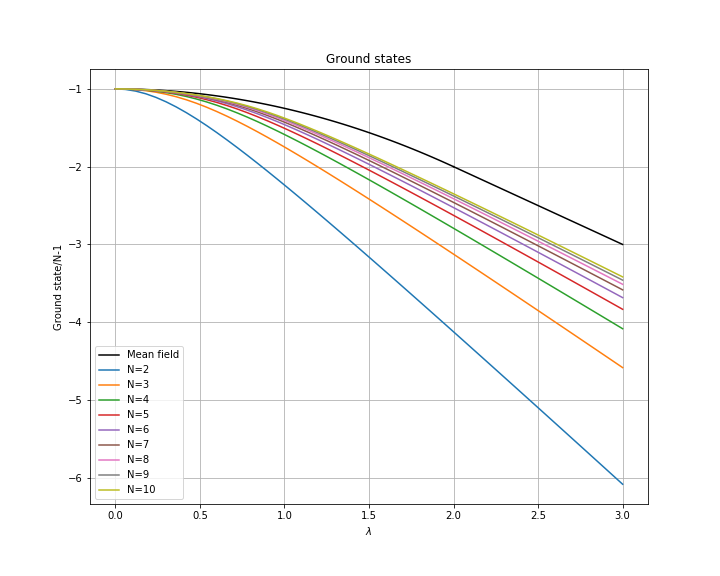
\includegraphics[width=\linewidth]{images/groundstates.png}
	\end{figure}
\end{center}
The computed ground states seem to look, as $N$ highers, more similar to the mean field solution. Below, instead, we show, for some $N$'s, the first four eigenvalues:
\begin{flushleft}
\begin{tabular}{ll}
	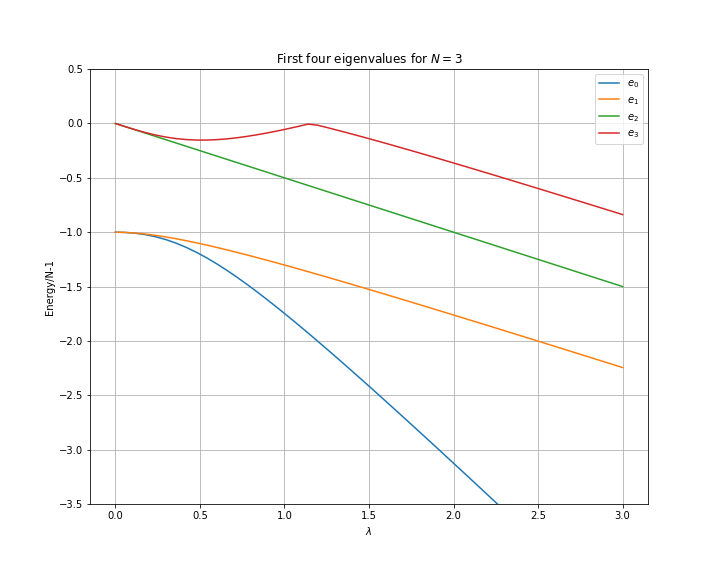
\includegraphics[width=0.65\linewidth,clip, trim={1.5cm 0 1.5cm 0}]{images/eigenvalues3.png} & 
	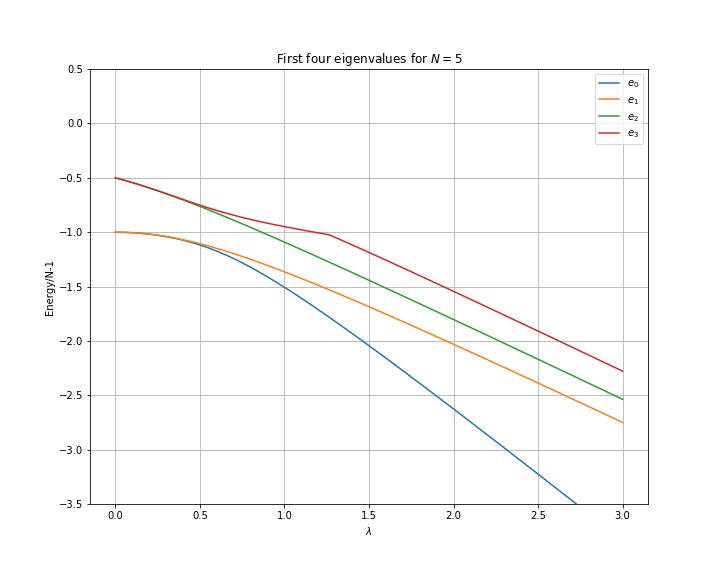
\includegraphics[width=0.65\linewidth,clip, trim={1.5cm 0 1.5cm 0}]{images/eigenvalues5.png} \\
	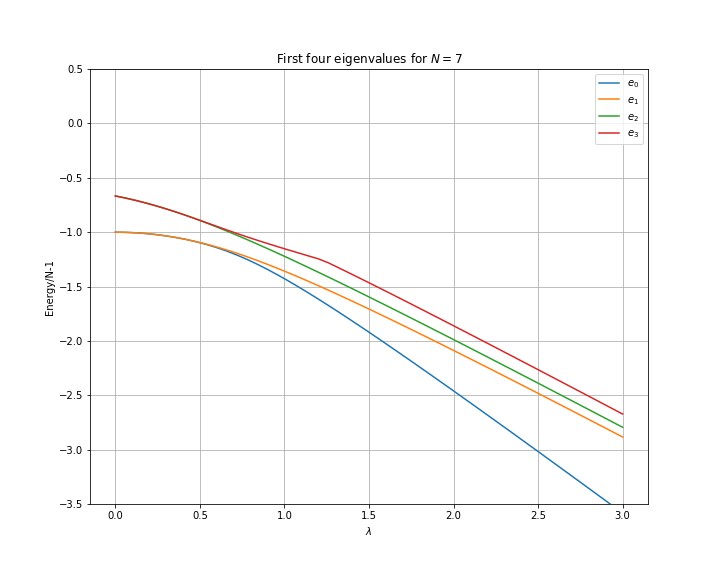
\includegraphics[width=0.65\linewidth,clip, trim={1.5cm 0 1.5cm 0}]{images/eigenvalues7.png} &
	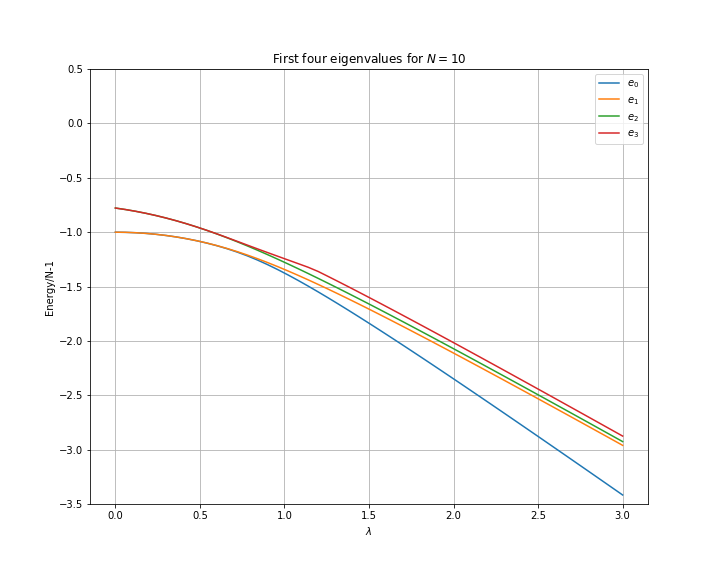
\includegraphics[width=0.65\linewidth,clip, trim={1.5cm 0 1.5cm 0}]{images/eigenvalues10.png}
\end{tabular}
\end{flushleft}
We can notice that as $N$ highers the ground state is more and more distinct form the other energy levels which tend to come closer, especially at higher $\lambda$'s.
Another related interesting phenomenon that we observe is the degeneracy removal,due to leaving $\lambda=0$.
\end{document}